\section{Characterization}\label{sec:characterization}

Magnetic characterization of flat curved structures utilizes the different methods, that could be generalized in the following groups:

\subsection{Magnetometry techniques}

This methods rely on measurements of magnetic responses from the curvilinear structures. Firstly, to this group should be included \textit{integral magnetometry} techniques, that provide the magnetic responses over the large-scale area and include the standard superconducting quantum interference device (SQUID) magnetometry, vibrating sample magnetometry (VSM) and magneto-optic Kerr effect (MOKE) magnetometry~\cite{Streubel12b,Streubel13c,Streubel14,Ueltzhoeffer16,Hunt20}, that recently was improved for high-precision analysis of curvilinear structures by utilizing dark-field MOKE magnetometry~\cite{Sanz-Hernandez17}, see Fig.~\ref{Fig:Experimental_figs_2}(a).

In addition to the integral methods, there is a group of \textit{local magnetometry} techniques  of the individual object, that retrieve both the spatial distribution of the stray fields and magnetic properties. This group includes dynamic cantilever-based~\cite{Degen09,Weber12,Mehlin18,Braakman19} (Fig.~\ref{Fig:Experimental_figs_2}(b)) and nano-SQUID magnetometries~\cite{Vasyukov18} (Fig.~\ref{Fig:Experimental_figs_2}(c)). Here it should be referred the scanning reconfigurable magnetic force microscopy (MFM)~\cite{Kazakova19,May19,Corte-Leon19}, that allows to quantify the 3D magnetization pattern of a magnetic nanoobject from a 2D data~\cite{Vock14}, and micro-Hall magnetometry that was applied for magnetic characterization of complex-shapes FEBID nanostructures~\cite{Keller18,Mamoori18} (Fig.~\ref{Fig:Experimental_figs_2}(d)). 

\begin{figure*}
	\centering
	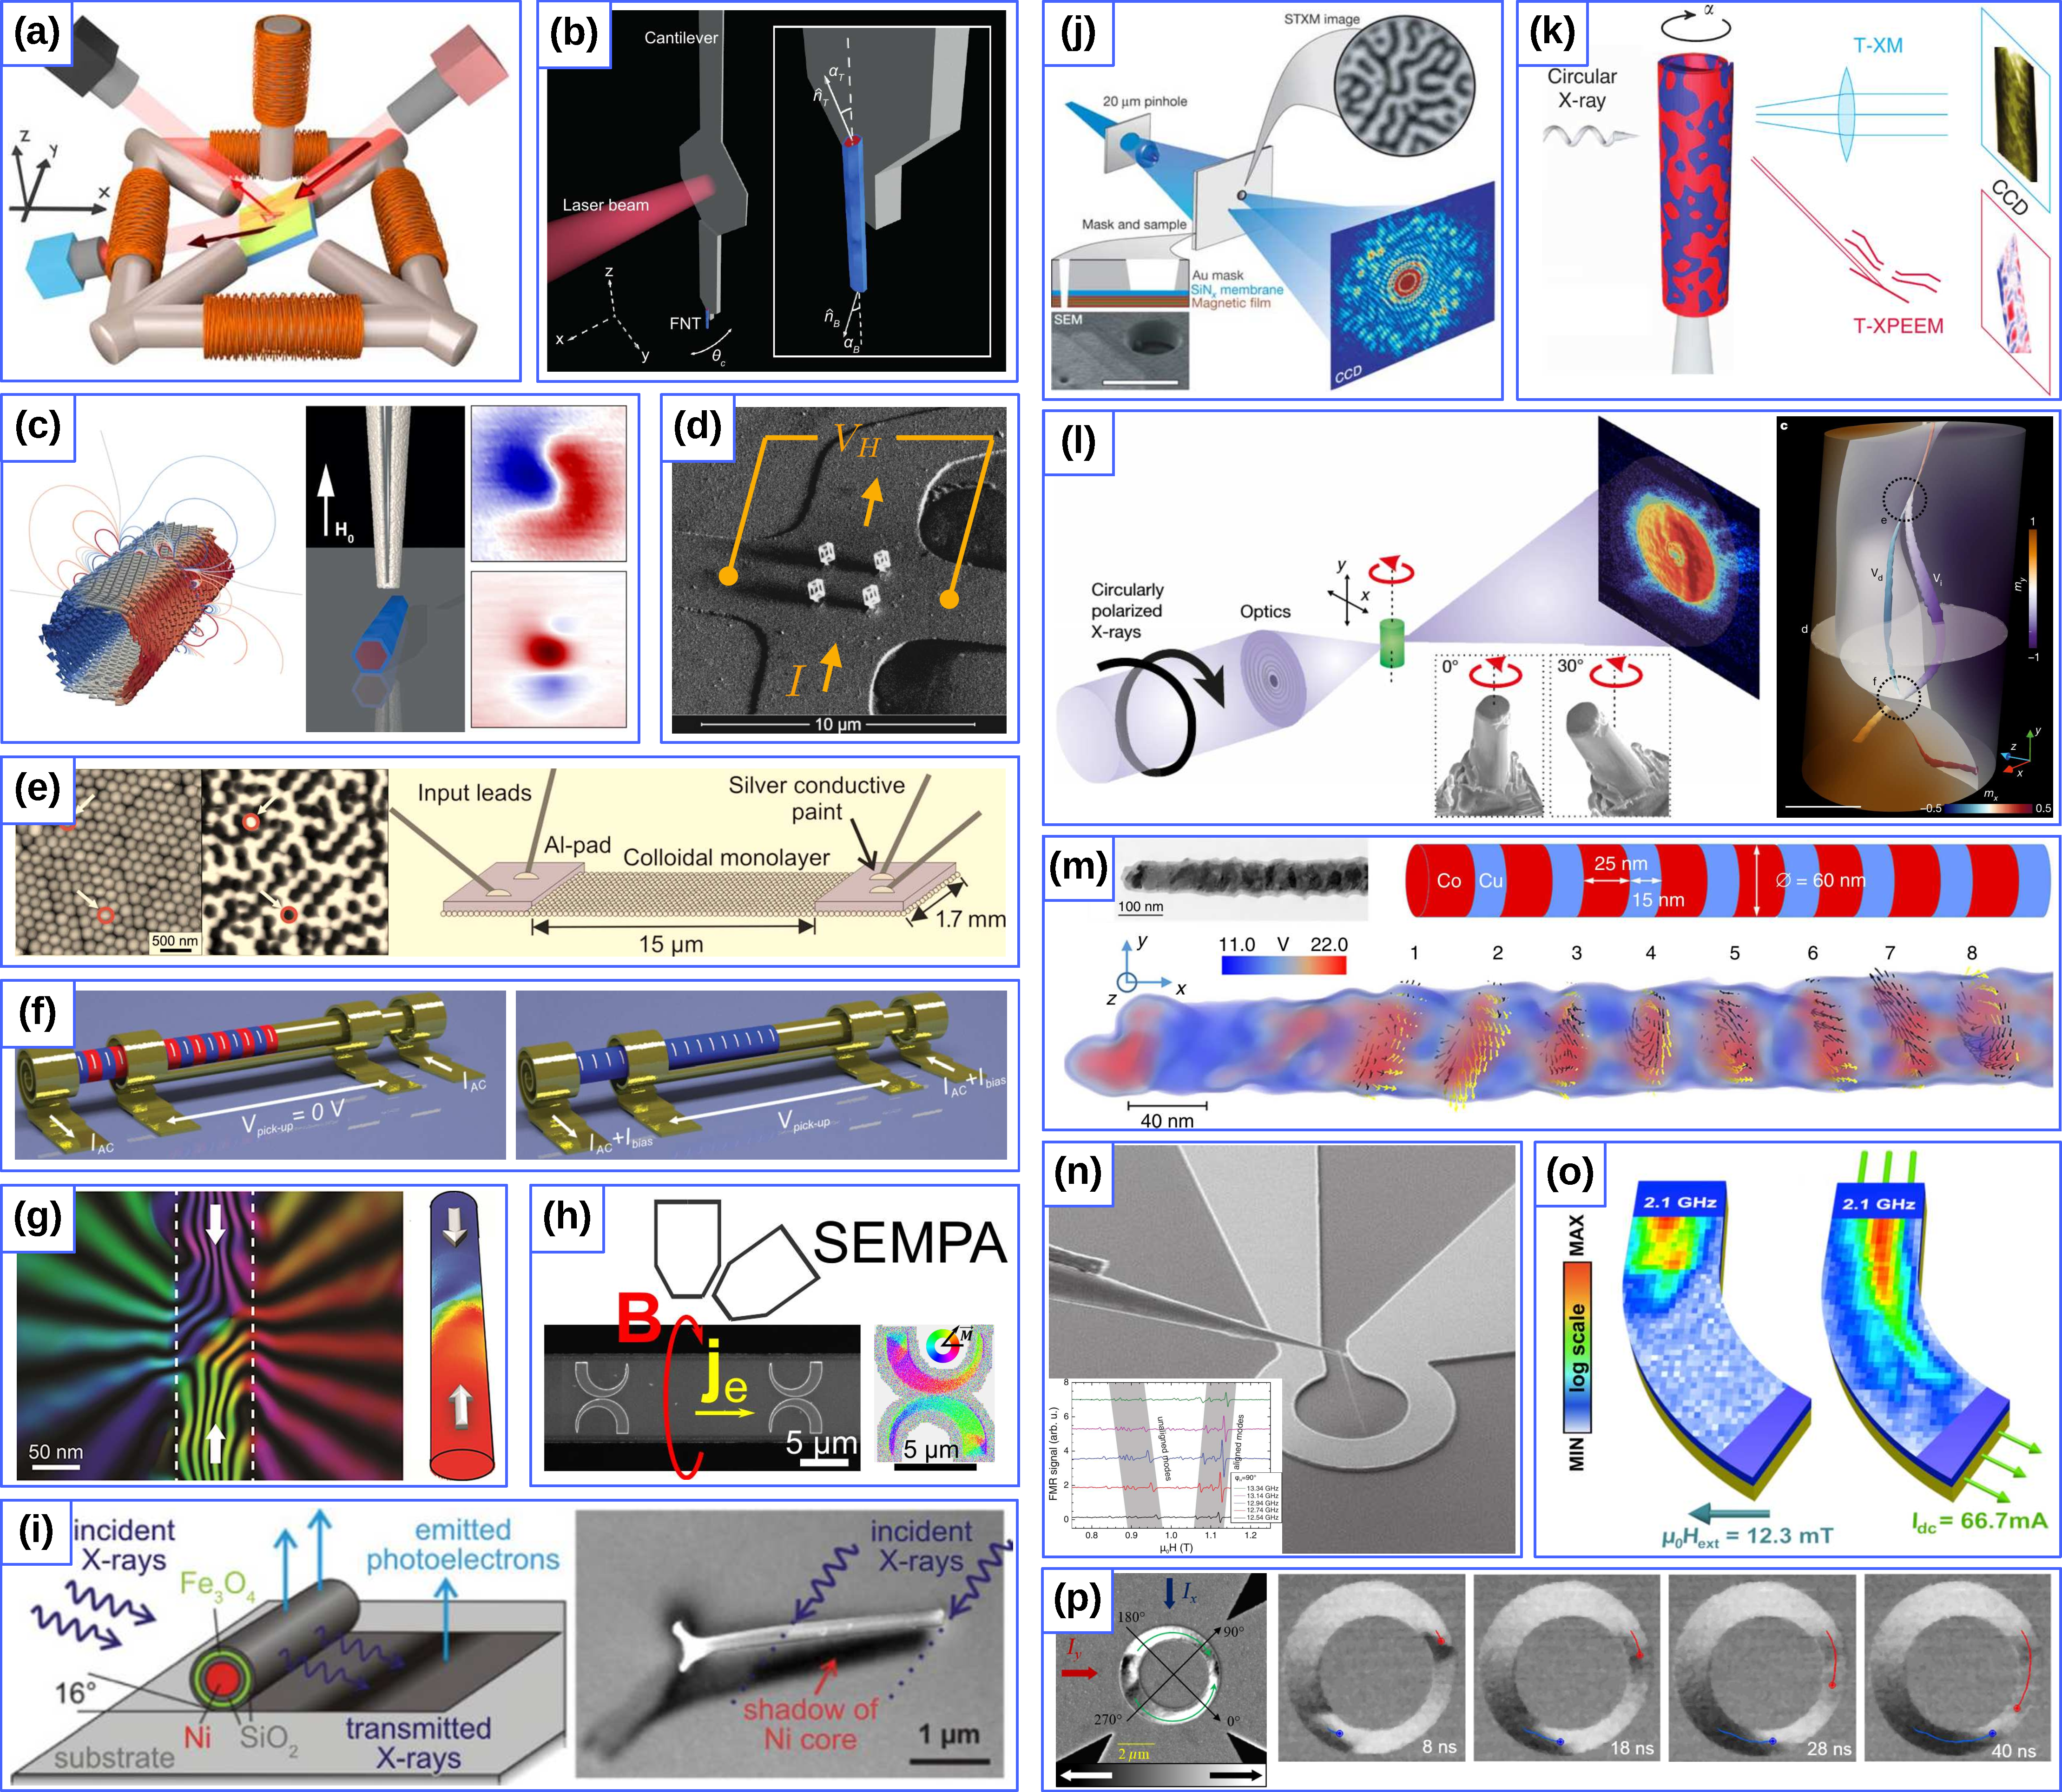
\includegraphics[width=0.97\linewidth]{fig_characterization.pdf}
	\caption{\textbf{Advanced characterization techniques for curvilinear nanomagnets.} \textbf{(a)} Schematics of dark-field MOKE. Adapted with permission from~\cite{Sanz-Hernandez17}. \textbf{(b)} Dynamic cantiliver-based magnetometry tip with magnetic nanotube at the end. Adapted with permission from~\cite{Mehlin18}. \textbf{(c)} Nano-SQUID tip and reconstructed stray field of hexagonal magnetic nanotube. Adapted with permission from~\cite{Vasyukov18}. \textbf{(d)} Micro-Hall cross setup with nanocubes. Adapted with permission from~\cite{Mamoori18}. \textbf{(e)} Sketch of AMR measurements on self-assembled magnetic nanoparticles. Adapted with permission from~\cite{KimlingnMoser10}. \textbf{(f)} Schematics of an integrated GMI sensor operation. Adapted with the permission from~\cite{Karnaushenko15a}. \textbf{(g)} Electron holography of a DW in Ni nanocylinder. Adapted with permission from~\cite{Biziere13}. \textbf{(h)} Sketch of SEMPA setup and color-coded image from flat curvilinear structures. Adapted with permission from~\cite{Schoenke20}. \textbf{(i)} XMCD-PEEM technique for 3D magnets with shadow contrast reconstruction. Adapted with permission from~\cite{Kimling11}. \textbf{(j)} (i) X-ray spectro-holography. Adapted with permission from~\cite{Eisebitt04}.
	\textbf{(k)} Concept of MXT based on a combination of STXM and XMCD-PEEM techniques for the 3D magnets. Adapted with permission from~\cite{Streubel15a}. \textbf{(l)} Hard X-Ray magnetic tomography setup based on ptychographic scans of a sample. Adapted with permission from~\cite{Donnelly17}.	\textbf{(m)} Holographic vector field electron tomography of 3D nanomagnets. Adapted with permission from~\cite{Wolf19}. \textbf{(n)} FMR measurements of a magnetic nanowire in $\Omega$-shaped resonator. Adapted with permission from~\cite{Lenz19}. \textbf{(o)} BLS intensity distribution of spin waves in a curved stripe. Adapted with permission from~\cite{Vogt12}. \textbf{(p)} Asymmetric ferromagnetic ring and STXM snapshots of automotive DWs motion. Adapted with permission from~\cite{Mawass17}.} 
	\label{Fig:Experimental_figs_2}
\end{figure*}

\subsection{Transport techniques}

This group of techniques provide the insight into the charge and spin transport properties of magnetic materials. These techniques include the group of magneto-sensitive transport-based electrical measurements, that employs: anisotropic magnetoresistance (AMR) effect for nanotubes~\cite{Rueffer12,Zimmermann18}, monolayer of magnetic spherical caps~\cite{KimlingnMoser10} (Fig.~\ref{Fig:Experimental_figs_2}(e)), ferromagnetic microhelices~\cite{Maurenbrecher18} and nanomembranes~\cite{Moench11,Schumann12,Muller12}; giant magnetoresistive (GMR) effect for nanomembranes~\cite{Mueller12}; giant magnetoimpedance (GMI) effect~\cite{Karnaushenko15a} Fig.~\ref{Fig:Experimental_figs_2}(f); current-induced spin torques~\cite{Schoebitz19}. 

\subsection{Magneto-sensitive visualization techniques}

A valuable information about the magnetization textures of curvilinear objects can be obtained by magneto-sensitive visualization techniques, that provide access to complex magnetization patterns on curved magnetic systems. These techniques include \textit{scanning-probe methods}, e.g. MFM, that provide a spatial resolution up to 50~nm for curved nanoobjects~\cite{Ulbrich06,Makarov07,Makarov08,Makarov09,Schulze10,Albrecht12,Nguyen15,Streubel16,Ball17,May19}; MOKE microscopy~\cite{Streubel12b,Streubel13c,Streubel14,Ueltzhoeffer16,Hunt20}, that recently was enabled for pump-probe time-resolved measurements of micro-tetrapod geometries~\cite{Sahoo18}; electron-based methods, including Lorentz transmission electron microscopy (TEM)~\cite{Phatak12,Phatak11} with its extension to electron holography, that allows to perform the detail static reconstruction of magnetic textures in flat~\cite{Klaeui05,Nord19} and 3D~\cite{Biziere13,Phatak14,Phatak20} curved geometries, see Fig.~\ref{Fig:Experimental_figs_2}(g); scanning electron technique with polarization analysis~(SEMPA)~\cite{Schoenke18}, that is suitable for imaging flat curved magnetic geometries~\cite{Klaui05,Schoenke20}, see Fig.~\ref{Fig:Experimental_figs_2}(h); X-ray-based visualization methods, including X-ray magnetic circular dichroism photoelectron emission microscopy (XMCD-PEEM)~\cite{Streubel15c,Streubel15,Streubel16,Volkov19,Volkov19c}.  

While these methods are limited to the analysis of simple magnetic geometries, the visualization of complex 3D shape geometries requires the utilization of the tomographic-based approaches. Thus, MOKE microscopy~\cite{Streubel14}, that recently was enabled for tomography-like screening of bulk samples~\cite{Schaefer20}; XMCD-PEEM was successfully extended to image interior magnetization textures of complex curved magnetic nanoobjects by using transmission shadow contrasts~\cite{Kimling11,Streubel12,Streubel12b,Streubel14a,DaCol14,Stano18a,Wartelle18,Schoebitz19,Wartelle19}, see Fig.~\ref{Fig:Experimental_figs_2}(i). X-ray spectro-holography~\cite{Eisebitt04} could be also utilizes for the characterization of 3D curved magnetic nanostructures (Fig.~\ref{Fig:Experimental_figs_2}(j)), e.g. magnetically capped nanospheres~\cite{Guenther10}. Full field X-ray microscopy, that combines magnetic transmission
soft X-ray microscopy (MXTM) with XMCD-PEEM, was successfully applied to realize the concept of soft X-ray magnetic tomography (MXT)~\cite{Streubel15a}, see Fig.~\ref{Fig:Experimental_figs_2}(k). Complementary, hard X-ray magnetic tomography with ptychographic scans potentially allows for 10 nm resolution of 3D magnetic textures~\cite{Donnelly17}, see Fig.~\ref{Fig:Experimental_figs_2}(l). The electron holography is extended to holographic vector field electron tomography~\cite{Wolf13,Wolf19}, see Fig.~\ref{Fig:Experimental_figs_2}(m), that allows to reconstruct 3D magnetic textures with a sub 10~nm resolution. 

\subsection{Dynamic magnetization methods}

Other methods, that rely on time domain and provide input on magnetization characterization are dynamic methods. These techniques include the ferromagnetic resonance (FMR) methods~\cite{Liedke13}, whose sensitivity for the study of curved magnetic objects could be substantially improved by utilizing microresanator loops~\cite{Lenz19}, see Fig.~\ref{Fig:Experimental_figs_2}(n). Another valuable dynamic measurement method is Brillouin light spectroscopy (BLS)~\cite{Demokritov01}, that recently was improved by using high-sensitive BLS microscopy~\cite{Vogt12,Vogt14,Schultheiss19}, see Fig.~\ref{Fig:Experimental_figs_2}(o). Also, it should be mentioned the possibility to perform dynamic magnetic imaging using scanning transmission X-ray microscope (STXM)~\cite{Wintz11,Streubel15,Streubel15d,Wintz16,Woo16,Zimmermann18,Sluka19}, see Fig.~\ref{Fig:Experimental_figs_2}(p).



%These techniques include the scanning-probe near-field methods, that are represented by: scanning reconfigurable magnetic force microscopy (MFM)~\cite{Kazakova19,May19,Corte-Leon19}, nano-superconducting quantum interference device magnetometry~\cite{Vasyukov18} and dynamic cantilever magnetometries~\cite{Degen09,Weber12,Mehlin18,Braakman19}. These methods allow to retrieve the magnetic properties and magnetization configuration from the demagnetizing fields of curvilinear structures. To the magnetometry techniques should be also included the group of magneto-sensitive transport-based electrical measurements, that employs: anisotropic magnetoresistance (AMR) effect for nanotubes~\cite{Rueffer12,Zimmermann18}, monolayer of magnetic spherical caps~\cite{KimlingnMoser10}, ferromagnetic microhelices~\cite{Maurenbrecher18} and nanomembranes~\cite{Moench11,Schumann12,Muller12}; giant magnetoresistive (GMR) effect for nanomembranes~\cite{Mueller12}; giant magnetoimpedance (GMI) effect~\cite{Karnaushenko15a}; micro-Hall magnetometry that was applied for magnetic characterization of complex-shapes FEBID nanostructures~\cite{Keller18,Mamoori18}; current-induced spin torques~\cite{Schoebitz19} and spin-orbit torques~~\cite{Miron10,Miron11a,Garello13,Manchon19}; magneto-optic Kerr effect (MOKE) magnetometry~\cite{Streubel12b,Streubel13c,Streubel14,Ueltzhoeffer16,Hunt20}, that recently was improved for high-precision analysis of curvilinear structures by utilizing dark-field MOKE magnetometry~\cite{Sanz-Hernandez17}.




% To these techniques should be also referred the mentioned above \textit{scanning-probe methods}, including MFM, that provide a spatial resolution up to 50~nm for curved nanoobjects~\cite{Ulbrich06,Makarov07,Makarov08,Makarov09,Schulze10,Albrecht12,Nguyen15,Streubel16,Ball17,May19}. MOKE microscopy~\cite{Streubel14}, that recently was enabled for tomography-like screening of bulk samples~\cite{Schaefer20} and pump-probe time-resolved measurements of micro-tetrapod geometries~\cite{Sahoo18}. The high-resolution magnetic imaging of curved geometries is achieved by means of different X-ray-based visualization methods, including X-ray magnetic circular dichroism photoelectron emission microscopy (XMCD-PEEM)~\cite{Streubel15c,Streubel15,Streubel16,Volkov19,Volkov19c}, that was successfully extended to image interior magnetization textures of complex curved magnetic nanoobjects by using transmission shadow contrasts~\cite{Kimling11,Streubel12,Streubel12b,Streubel14a,Wartelle18,Schoebitz19,Wartelle19}, see Fig.~\ref{Fig:Experimental_figs_2}(b), and subsequently modified to the concept of soft X-ray magnetic tomography (MXT)~\cite{Streubel15a}, see Fig.~\ref{Fig:Experimental_figs_2}(c), and hard X-ray magnetic tomography with ptychographic scans potentially allows for 10 nm resolution of 3D magnetic textures~\cite{Donnelly17}, see Fig.~\ref{Fig:Experimental_figs_2}(a). It should be mentioned also the possibility to utilize the X-ray spectro-holography~\cite{Eisebitt04} for the characterization of microscopic magnetically capped nanospheres~\cite{Guenther10}. Another valuable imaging techniques are electron-based methods, including scanning electron technique with polarization analysis~(SEMPA)~\cite{Schoenke18}, that is suitable for imaging flat curved magnetic geometries~\cite{Klaui05,Schoenke20}, Lorentz transmission electron microscopy (TEM)~\cite{Phatak12,Phatak11} with its extension to electron holography, that allows to perform the detail static reconstruction of magnetic textures in flat~\cite{Klaeui05,Nord19} and 3D~\cite{Phatak14,Phatak20} curved geometries, and its further extension to holographic vector field electron tomography~\cite{Wolf13,Wolf19}, see Fig.~\ref{Fig:Experimental_figs_2}(d), that allows to reconstruct 3D magnetic textures with a sub 10~nm resolution.


%The \textbf{characterization of magnetic responses} from 3D curvilinear objects utilizes (I) a high-resolution magneto-sensitive visualization techniques, that enable a direct reconstruction of the magnetization distribution in 3D object,  and (II) advanced magnetometry techniques, that indirectly infer the magnetic configuration of nanosctructure, as demonstrated in Fig.~\ref{Fig:Experimental_figs_2}. The first type of techniques is based on the high-resolution vector tomography, e.g. the hard X-Ray magnetic tomography with ptychographic scans potentially allows for 10 nm resolution of 3D magnetic textures~\cite{Donnelly17}, see Fig.~\ref{Fig:Experimental_figs_2}(a). Soft X-Ray magnetic circular dichroism photoelectron emission microscopy (XMCD-PEEM) was successfully applied to image interior domain patterns in nanorods relying on a transmission shadow contrast~\cite{Kimling11}, see Fig.~\ref{Fig:Experimental_figs_2}(b). This method was modified to the concept of soft X-ray magnetic tomography (MXT)~\cite{Streubel15a}, see Fig.~\ref{Fig:Experimental_figs_2}(c). Another valuable tomographic method, that allows to reconstruct magnetic textures with a sub 10 nm resolution, is holographic vector field electron tomography~\cite{Wolf13,Wolf19}, see Fig.~\ref{Fig:Experimental_figs_2}(d). It should be mentioned also the possibility to utilize the X-ray spectro-holography~\cite{Eisebitt04} for the characterization of microscopic magnetically capped nanospheres~\cite{Guenther10}. 

%The second type of experimental methods relies on the novel magnetometry techniques, that rely on the indirect measurements of magnetic responses from the curvilinear structures. There are optical, electrical and near-field high-sensitive magnetometry methods. The first type of magnetometry techniques is based on the magnetooptical Kerr effect (MOKE) and Brillouin light spectroscopy (BLS)~\cite{Demokritov01} methods. Recently, the standard MOKE was developed for high-precision analysis of curvilinear structures by utilizing dark-field MOKE magnetometry~\cite{Sanz-Hernandez17}, pump-probe time-resolved MOKE measurements~\cite{Sahoo18}  and tomography-like MOKE screening of bulk samples~\cite{Schaefer20}, while the convenient BLS method was improved by using high-sensitive BLS microscopy~\cite{Vogt12,Vogt14,Schultheiss19}. The group of electrical magnetometry techniques is based on the resistance measurements of magnetic samples in external field, that employs magnetoresistance~\cite{KimlingnMoser10,Maurenbrecher18}, micro-Hall~\cite{Keller18,Mamoori18} effects and current-induced spin-orbit torques in magnetic systems~\cite{Miron10,Miron11a,Garello13,Manchon19}. The near-field magnetometry method are represented by a scanning reconfigurable magnetic force microscopy (MFM)~\cite{Kazakova19,May19,Corte-Leon19}, nano-superconducting quantum interference devices~\cite{Vasyukov18} and dynamic cantilever magnetometries~\cite{Mehlin18}. 